\documentclass{amsart}

\usepackage{amsfonts,amssymb,amscd,amsmath,enumerate,verbatim, calc,xypic, appendix, tikz, float}
\usepackage{graphicx, chngpage, mathtools,longtable, listings}
\usetikzlibrary{fit, arrows, automata}
\graphicspath{{./images/}} \tolerance=1000 \CompileMatrices

\newcommand{\centered}[1]{\begin{tabular}{l} #1 \end{tabular}}



\newcommand{\sss}{\scriptscriptstyle}
\newcommand{\ges}{\operatorname{\sss\geqslant}}
\newcommand{\les}{\operatorname{\sss\leqslant}}
\newcommand{\sges}{\operatorname{\sss>}}
\newcommand{\sles}{\operatorname{\sss<}} \newcommand{\maxi}{\operatorname
{\max}} \newcommand{\cls}[1]{{\operatorname{cls}(#1)}}
\newcommand{\col}{\colon}
\newcommand{\dd}{\partial}
\newcommand{\HH}[2]{\operatorname{H}_{#1}(#2)}
\newcommand{\Ker}{\operatorname{Ker}} \newcommand{\Coker}{\operatorname{Coker}}
\newcommand{\ds}{\operatorname{\displaystyle}}
\newcommand{\chr}{\operatorname{char}}
\newcommand{\la}{\operatorname{\!\langle\!}}
\newcommand{\lra}{\longrightarrow}
\newcommand{\pd}[2]{\operatorname{pd}_{#1}{#2}}
\newcommand{\rank}{\operatorname{rank}} \newcommand{\Hom}{\operatorname{Hom}}
\newcommand{\Gdim}[2]{\operatorname{G-dim}_{#1}{#2}}
\newcommand{\Hdim}[2]{{\operatorname{G}{\!}^*{\!}\operatorname{-dim}_{#1}{#2}}}
\newcommand{\Cdim}[2]{\operatorname{CI-dim}_{#1}{#2}}
\newcommand{\PCIdim}[2]{{\operatorname{CI}{\!}_*{\!}\operatorname{-dim}_{#1}{#2}}}
\newcommand{\CMdim}[2]{\operatorname{CM-dim}_{#1}{#2}}
\newcommand{\hdim}[2]{\operatorname{H-dim}_{#1}{#2}}
\newcommand{\Pdim}[2]{\operatorname{P-dim}_{#1}{#2}}
\newcommand{\Tor}[4]{\operatorname{Tor}_{#1}^{#2}(#3,#4){}}
\newcommand{\Ext}[4]{\operatorname{Ext}_{#1}^{#2}(#3,#4){}}
\newcommand{\var}{{\hskip1pt\vert\hskip1pt}}
\newcommand{\depth}[2]{\operatorname{depth}_{#1}{#2}}
\newcommand{\edim}{\operatorname{edim}}
\newcommand{\codepth}{\operatorname{codepth}}
\newcommand{\dime}{\operatorname{dim}}
\newcommand{\grade}[2]{\operatorname{grade}_{#1}{#2}}
\newcommand{\xra}{\xrightarrow}
\newcommand{\cx}[2]{\operatorname{cx}_{#1}{#2}}
\newcommand{\infe}{\operatorname{inf}} \newcommand{\supr}{\operatorname{sup}}
\newcommand{\card}{\operatorname{card}} \newcommand{\Supp}[2]{\operatorname
{Supp}_{#1}{(#2)}} \newcommand{\ann}{\operatorname{ann}}
\newcommand{\syz}[3]{\operatorname{Syz}_{#1}^{#2}{(#3)}}
\newcommand{\ba}{{\boldsymbol a}} \newcommand{\bX}{{\boldsymbol X}}
\newcommand{\bB}{{\boldsymbol B}} \newcommand{\bC}{{\boldsymbol C}}
\newcommand{\bF}{{\boldsymbol F}} \newcommand{\BF}{{\mathbb F}}
\newcommand{\BN}{{\mathbb N}} \newcommand{\BZ}{{\mathbb Z}}
\newcommand{\bsb}{{\boldsymbol b}} \newcommand{\bsy}{{\boldsymbol y}}
\newcommand{\bsf}{{\boldsymbol f}} \newcommand{\bsm}{{\boldsymbol m}}
\newcommand{\bsn}{{\boldsymbol n}} \newcommand{\bsp}{{\boldsymbol p}}
\newcommand{\bsq}{{\boldsymbol q}} \newcommand{\bss}{{\boldsymbol s}}
\newcommand{\bsx}{{\boldsymbol x}}
\newcommand{\E}[2]{\operatorname{E}^{#1}_{#2}} \newcommand{\im}{\operatorname
{Im}} \newcommand{\md}{{\displaystyle}}

\newtheorem{theorem*}{Main Theorem}

\newtheorem{theorem}{Theorem}[section]
\theoremstyle{theorem}
\theoremstyle{theorem*}
\newtheorem{corollary}[theorem]{Corollary}
\newtheorem{lemma}[theorem]{Lemma}
\newtheorem{proposition}[theorem]{Proposition}
\newtheorem{question}[theorem]{Question}
\newtheorem{partt}{Part}
\theoremstyle{definition}
\newtheorem{chunk}[theorem]{}
\newtheorem{schunk}[theorem]{}
\newtheorem{example}[theorem]{Example}
\newtheorem{examples}[theorem]{Examples}
\newtheorem{remark}[theorem]{Remark}
\newtheorem{computation}[theorem]{Computation}
\newtheorem{notation}[theorem]{Notation}
\newtheorem{definition}{Definition}
\begin{document}

\date{\today}
\title[Euler Matrices and Mahler Measure] {Euler Matrices of Quivers and Mahler Measure}
\author[T. Nichols]{Ty Nichols}
\address{Department of Mathematics, Northeastern University, Boston,
    Massachusetts~02115}
\email{nichols.t@northeastern.edu}
\begin{abstract} For a given quiver $Q$, we can define the matrix $B$ such that
    $B = -(E^T)E^{-1}$, where $E$ is the Euler matrix of $Q$. We will
    investigate the Mahler measure of the characteristic polynomial of $B$ for
    small quivers, paying particular attention to quivers whose underlying graph
    is close to being a simply laced Dynkin diagram or an extended Dynkin
    diagram. We hope to use properties of $B$ to investigate Lehmer's
    Conjecture. For this project, we will be working with Professor Harm
    Derksen.
\end{abstract}
\maketitle

\section{Introduction}

We begin by introducing basic terminology that motivates our approach to the
problem. The main objects under study are quivers, and the related matrices are
defined for use in the theory of quiver representations.

\subsection{Quivers}

\begin{definition} \cite{dw} A \textit{quiver} $Q$ is a 4-tuple $Q = (Q_0, Q_1,
        h, t)$ where $Q_0$ is a finite set of vertices, $Q_1$ is the set of
    edges, and $h: Q_1 \rightarrow Q_0$ and $t : Q_1 \rightarrow Q_0$ are
    functions that give the head and tail of each edge, respectively.
\end{definition}

\begin{definition} \cite{dw} A \textit{path} on a quiver $Q = (Q_0, Q_1, h, t)$
    from $u$ to $v$ for $u, v \in Q_0$ is some sequence of edges $e_0, \dots
        e_n$ such that for $0 \leq i \leq n$, $h(e_{i-1}) = t(e_i)$ and $t(e_0) =
        u$, $h(e_n) = v$.
\end{definition}

\begin{example}
    Consider the quiver illustrated by the following diagram:

    $$
        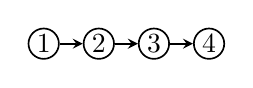
\begin{tikzpicture}[
                > = stealth, % arrow head style
                % shorten > = 1pt, % don't touch arrow head to node
                auto,
                node distance = 7mm, % distance between nodes
                semithick % line style
            ]

            \tikzstyle{every node}=[
            draw = black,
            circle,
            inner sep = 1pt,
            minimum size = 0.1mm
            ]

            \node (1) {$1$};
            \node (2) [right of=1] {$2$};
            \node (3) [right of=2] {$3$};
            \node (4) [right of=3] {$4$};

            \path[->] (1) edge (2);
            \path[->] (2) edge (3);
            \path[->] (3) edge (4);
        \end{tikzpicture}
    $$

    Then $Q_0 = \{1, 2, 3, 4\}$, $Q_1 = \{(1,2), (2,3), (3,4) \}$, and $h((1,2))
        = 2$ while $t((1,2)) = 1$.
\end{example}

\begin{example}
    Consider

    $$
        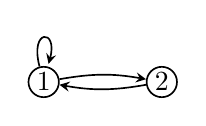
\begin{tikzpicture}[
                > = stealth, % arrow head style
                % shorten > = 1pt, % don't touch arrow head to node
                auto,
                node distance = 15mm, % distance between nodes
                semithick % line style
            ]

            \tikzstyle{every node}=[
            draw = black,
            circle,
            inner sep = 1pt,
            minimum size = 0.1mm
            ]

            \node (1) {$1$};
            \node (2) [right of=1] {$2$};

            \path[->, bend left=10] (1) edge (2);
            \path[->, bend left=10] (2) edge (1);
            \path[->] (1) edge [loop above] (1);
        \end{tikzpicture}
    $$

    Then $Q_0 = \{1, 2\}$, $Q_1 = \{(1,2), (2,1), (1,1) \}$, and $h((1,1)) =
        t((1,1)) = 1$.
\end{example}

Notice that self-loops and cycles are permitted, and that the functions $h$ and
$t$ are not necessarily injective, i.e. edges with the same head and tail may be
repeated. However, we will be considering quivers that do not contain
\textit{oriented cycles}:

\begin{definition} \cite{dw} An \textit{oriented cycle} of a quiver $Q = (Q_0,
        Q_1, h, t)$ is a path from $u$ to $u$. Notice that we may equivalently
    say that the cycle is a path from $v$ to $v$ for any $v$ contained in
    the cycle.
\end{definition}

\begin{example}
    Consider again the quivers in Examples 0.1 and 0.2. Observe that the quiver
    in example 0.1 does not contain an oriented cycle, as there is no path from
    any node back to itself. However, the quiver in example 2 contains multiple
    oriented cycles; one consists only of the self-loop on 1, while the other
    consists of the edges $(1,2)$ and $(2,1)$.
\end{example}

\subsection{Quiver Representations}

The matrices under study for this project are defined in the study of quiver
representations, which can be formally described as the following:

\begin{definition} \cite{dw} A \textit{representation} $V$ of a quiver $Q$ is a
    map $V_0$ that assigns a finite dimensional vector space to every vertex in
    $Q_0$, and for every edge $a \in Q_1$, an assignment of a linear
    transformation $V_a : V_0(t(a)) \rightarrow V_0(h(a))$.
\end{definition}

Of interest in representation theory is the Euler Matrix of a quiver:

\begin{definition} \cite{dw} Given a quiver $Q = (Q_0, Q_1, h, t)$, then the
    \textit{Euler matrix} $E$ of $Q$ is defined as

    $$E_{i,j} = \delta_{i,j} - |\{a \in Q_1 : t(a) = i, h(a) = j \}|$$

    where $\delta_{i,j}$ is the Kronecker symbol, defined as

    $$\delta_{i,j} = \begin{cases} 1 \text{ if } i = j \\ 0 \text{ if } i \neq j
            \\\end{cases}$$

\end{definition}

\subsection{Ausland-Reiter Transform}

This project studies the matrix product defined by $B = -E^T E^{-1}$, where $E$
is the Euler Matrix for some quiver $Q$. The matrix $B$ is used in the
Ausland-Reiter Transform \cite{dw}; however, defining the transform is currently
beyond the scope of this project.
\subsection{Dynkin Diagrams}

Of particular importance in representation theory are the \textit{Dynkin
    diagrams}, which are related to irreducible root systems and Lie algebras
\cite{dw}. Many of the connections in which these diagrams appear are beyond
the scope of this paper, but the diagrams themselves will be important, so
we provide them below.

\begin{definition} \cite{dw}

    The \textit{simply laced Dynkin diagrams} are $A_n, D_n, E_6, E_7, $ and
    $E_8$ \cite{dw}. Dynkin diagrams are typically drawn as undirected graphs;
    if we speak of a quiver as being related to a Dynkin diagram, we mean the
    quiver drawn also as an undirected graph.

    $$                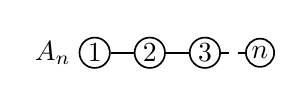
\begin{tikzpicture}[> = stealth, % arrow head style
                % shorten > = 1pt, % don't touch arrow head to node
                auto, node distance = 7mm, % distance between nodes
                semithick % line style
            ]

            \tikzstyle{every node}=[draw = black, circle, inner sep = 1pt,
            minimum size = 1mm]

            \node (1) [label=left:$A_n$] {$1$}; \node (2) [right of=1] {$2$};
            \node (3) [right of=2] {$3$}; \node (4) [right of=3] {$n$};

            \path[-] (1) edge (2); \path[-] (2) edge (3); \path[dashed] (3) edge
            (4);

        \end{tikzpicture}
    $$

    $$                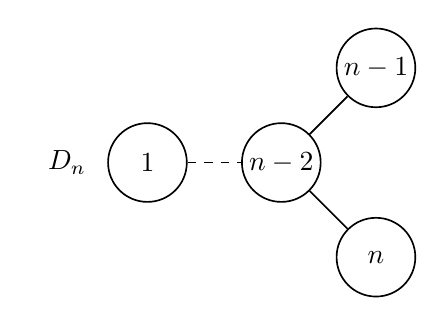
\begin{tikzpicture}[
                > = stealth, % arrow head style
                % shorten > = 1pt, % don't touch arrow head to node
                auto, node distance = 17mm, % distance between nodes
                semithick % line style
            ]

            \tikzstyle{every node}=[draw = black, circle, inner sep = 1pt,
            minimum size = 1cm]

            \node (1) [label=left:$D_n$] {$1$}; \node (2) [right of=1] {$n-2$};
            \node (3) [above right of=2] {$n-1$}; \node (4) [below right of=2]
            {$n$};

            \path[dashed] (1) edge (2); \path[-] (2) edge (3); \path[-] (2) edge
            (4);

        \end{tikzpicture}
    $$

    $$                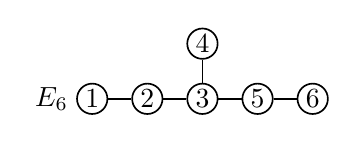
\begin{tikzpicture}[
                > = stealth, % arrow head style
                % shorten > = 1pt, % don't touch arrow head to node
                auto, node distance = 7mm, % distance between nodes
                semithick % line style
            ]

            \tikzstyle{every node}=[draw = black, circle, inner sep = 1pt,
            minimum size = 0.1mm]

            \node (1) [label=left:$E_6$] {$1$}; \node (2) [right of=1] {$2$};
            \node (3) [right of=2] {$3$}; \node (4) [above of=3] {$4$}; \node
            (5) [right of=3] {$5$}; \node (6) [right of=5] {$6$};

            \path[-] (1) edge (2); \path[-] (2) edge (3); \path[-] (3) edge (4);
            \path[-] (3) edge (5); \path[-] (5) edge (6);

        \end{tikzpicture}
    $$

    $$                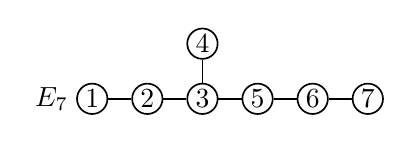
\begin{tikzpicture}[
                > = stealth, % arrow head style
                % shorten > = 1pt, % don't touch arrow head to node
                auto, node distance = 7mm, % distance between nodes
                semithick % line style
            ]

            \tikzstyle{every node}=[draw = black, circle, inner sep = 1pt,
            minimum size = 0.1mm]

            \node (1) [label=left:$E_7$] {$1$}; \node (2) [right of=1] {$2$};
            \node (3) [right of=2] {$3$}; \node (4) [above of=3] {$4$}; \node
            (5) [right of=3] {$5$}; \node (6) [right of=5] {$6$}; \node (7)
            [right of=6] {$7$};

            \path[-] (1) edge (2); \path[-] (2) edge (3); \path[-] (3) edge (4);
            \path[-] (3) edge (5); \path[-] (5) edge (6); \path[-] (6) edge (7);

        \end{tikzpicture}
    $$

    $$                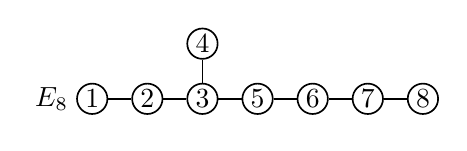
\begin{tikzpicture}[
                > = stealth, % arrow head style
                % shorten > = 1pt, % don't touch arrow head to node
                auto, node distance = 7mm, % distance between nodes
                semithick % line style
            ]

            \tikzstyle{every node}=[draw = black, circle, inner sep = 1pt,
            minimum size = 0.1mm]

            \node (1) [label=left:$E_8$] {$1$}; \node (2) [right of=1] {$2$};
            \node (3) [right of=2] {$3$}; \node (4) [above of=3] {$4$}; \node
            (5) [right of=3] {$5$}; \node (6) [right of=5] {$6$}; \node (7)
            [right of=6] {$7$}; \node (8) [right of=7] {$8$};

            \path[-] (1) edge (2); \path[-] (2) edge (3); \path[-] (3) edge (4);
            \path[-] (3) edge (5); \path[-] (5) edge (6); \path[-] (6) edge (7);
            \path[-] (7) edge (8);

        \end{tikzpicture}
    $$

    Also of interest are the \textit{extended Dynkin diagrams} $\hat{A}_n$, $\hat{D}_n$, $\hat{E}_6$, $\hat{E}_7$, and $\hat{E}_8$.

    $$                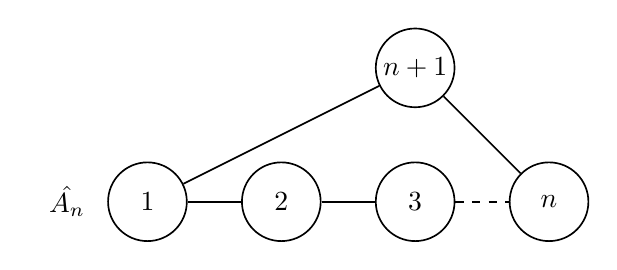
\begin{tikzpicture}[
                > = stealth, % arrow head style
                % shorten > = 1pt, % don't touch arrow head to node
                auto, node distance = 17mm, % distance between nodes
                semithick % line style
            ]

            \tikzstyle{every node}=[draw = black, circle, inner sep = 1pt,
            minimum size = 1cm]

            \node (1) [label=left:$\hat{A_n}$] {$1$}; \node (2) [right of=1]
            {$2$}; \node (3) [right of=2] {$3$}; \node (4) [right of=3] {$n$};
            \node (5) [above of=3] {$n+1$};

            \path[-] (1) edge (2); \path[-] (2) edge (3); \path[dashed] (3) edge
            (4); \path[-] (4) edge (5); \path[-] (1) edge (5);

        \end{tikzpicture}
    $$

    $$                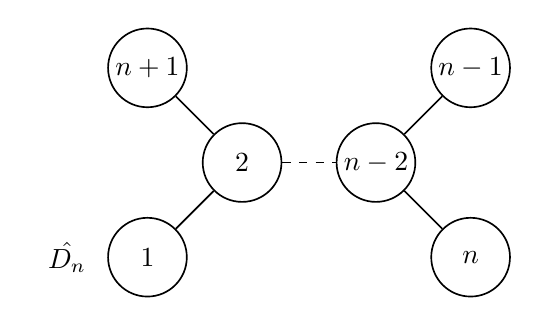
\begin{tikzpicture}[
                > = stealth, % arrow head style
                % shorten > = 1pt, % don't touch arrow head to node
                auto, node distance = 17mm, % distance between nodes
                semithick % line style
            ]

            \tikzstyle{every node}=[draw = black, circle, inner sep = 1pt,
            minimum size = 1cm]

            \node (1) {$2$}; \node (2) [above left of=1] {$n+1$}; \node (3)
            [label=left:$\hat{D_n}$][below left of=1] {$1$}; \node (4) [right
                of=1] {$n - 2$}; \node (5) [above right of=4] {$n - 1$}; \node (6)
            [below right of=4] {$n$};

            \path[-] (1) edge (2); \path[-] (1) edge (3); \path[dashed] (1) edge
            (4); \path[-] (4) edge (5); \path[-] (4) edge (6);


        \end{tikzpicture}
    $$

    $$                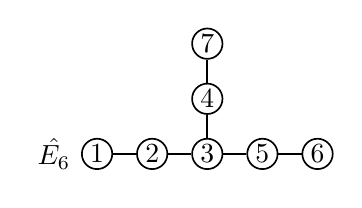
\begin{tikzpicture}[
                > = stealth, % arrow head style
                % shorten > = 1pt, % don't touch arrow head to node
                auto, node distance = 7mm, % distance between nodes
                semithick % line style
            ]

            \tikzstyle{every node}=[draw = black, circle, inner sep = 1pt,
            minimum size = 0.1mm]

            \node (1) [label=left:$\hat{E_6}$] {$1$}; \node (2) [right of=1]
            {$2$}; \node (3) [right of=2] {$3$}; \node (4) [above of=3] {$4$};
            \node (5) [right of=3] {$5$}; \node (6) [right of=5] {$6$}; \node
            (7) [above of=4] {$7$};

            \path[-] (1) edge (2); \path[-] (2) edge (3); \path[-] (3) edge (4);
            \path[-] (3) edge (5); \path[-] (5) edge (6); \path[-] (4) edge (7);

        \end{tikzpicture}
    $$

    $$                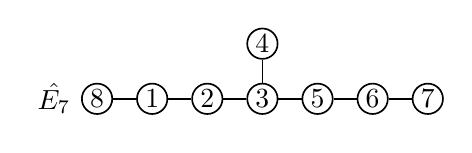
\begin{tikzpicture}[
                > = stealth, % arrow head style
                % shorten > = 1pt, % don't touch arrow head to node
                auto, node distance = 7mm, % distance between nodes
                semithick % line style
            ]

            \tikzstyle{every node}=[draw = black, circle, inner sep = 1pt,
            minimum size = 0.1mm]

            \node (1) {$1$}; \node (2) [right of=1] {$2$}; \node (3) [right
                of=2] {$3$}; \node (4) [above of=3] {$4$}; \node (5) [right
                of=3] {$5$}; \node (6) [right of=5] {$6$}; \node (7) [right
                of=6] {$7$}; \node (8) [label=left:$\hat{E_7}$][left of=1]
            {$8$};

            \path[-] (1) edge (2); \path[-] (2) edge (3); \path[-] (3) edge (4);
            \path[-] (3) edge (5); \path[-] (5) edge (6); \path[-] (6) edge (7);
            \path[-] (1) edge (8);

        \end{tikzpicture}
    $$

    $$                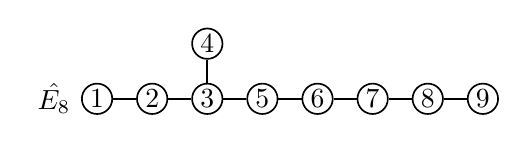
\begin{tikzpicture}[
                > = stealth, % arrow head style
                % shorten > = 1pt, % don't touch arrow head to node
                auto, node distance = 7mm, % distance between nodes
                semithick % line style
            ]

            \tikzstyle{every node}=[draw = black, circle, inner sep = 1pt,
            minimum size = 0.1mm]

            \node (1) [label=left:$\hat{E_8}$] {$1$}; \node (2) [right of=1]
            {$2$}; \node (3) [right of=2] {$3$}; \node (4) [above of=3] {$4$};
            \node (5) [right of=3] {$5$}; \node (6) [right of=5] {$6$}; \node
            (7) [right of=6] {$7$}; \node (8) [right of=7] {$8$}; \node (9)
            [right of=8] {$9$};

            \path[-] (1) edge (2); \path[-] (2) edge (3); \path[-] (3) edge (4);
            \path[-] (3) edge (5); \path[-] (5) edge (6); \path[-] (6) edge (7);
            \path[-] (7) edge (8); \path[-] (8) edge (9);

        \end{tikzpicture}
    $$

\end{definition}
According to professor Derksen, the eigenvalues of $B$ will lie on the unit circle when the quiver $Q$ is either a simply laced Dynkin diagram or an extended Dynkin diagram.
\subsection*{Mahler Measure}

We consider the \textit{Mahler Measure} of polynomials to evaluate "closeness" of their roots to the unit circle in the complex plane:

\begin{definition} \cite{m}

    Given a polynomial $P(x) \in \mathbb{Z}[x]$ with integer coefficients where $P(x) = a_n \Pi_{k=1}^{n} (x - \alpha_k)$, the \textit{Mahler Measure of P} is defined as

    $$M(P) = |a_d|\Pi_{k=1}^{n}\max\{1, |\alpha_k|\}$$

\end{definition}

We will also define for convenience the Mahler Measure of a matrix, which will
be the Mahler measure of its characteristic polynomial, and the Mahler measure
of a quiver, which will be the Mahler measure of its matrix $B$ when $E$ is not
singular.

For our matrix $B$, we may simplify the equation for Mahler measure slightly:

\begin{remark}
    Since the matrix $B$ has integer coefficients, its characteristic polynomial
    has integer coefficients, and since the characteristic polynomial has the
    eigenvalues of $B$ as roots, the leading factor $|a_d|$ will always be 1.
    This means that
    $$M(B) = \Pi_{k=1}^{n}\max\{1, |\lambda_k|\}$$
\end{remark}


Observe that the Mahler Measure of a matrix is very similar to the determinant
of that matrix, since $\det(B)$ is equal to the product of all eigenvalues of
$B$. Knowing this, we can compare them:
\begin{proposition}
    For any matrix $B$ with integer entries, $\det(B) \leq M(B)$.

    \begin{proof}
        Suppose an $n$x$n$ matrix $B$ has eigenvalues $\lambda_1, \dots
            \lambda_n$. Then $\det(B) = \lambda_1 \cdots \lambda_n$, so
        $|\det(b)| = |\lambda_1 \cdots \lambda_n| = |\lambda_1| \dots
            |\lambda_n|$. But since $M(B) = |\max\{1, \lambda_1\}| \dots
            |\max\{1, \lambda_n\}|$ and for any $\lambda_i$, $\lambda_i \leq
            \max\{1, \lambda_i\}$, it follows that $|\det(B)| \leq |M(B)|$.

        However, Mahler measure is defined to be a positive real number, and $B$
        has integer entries, so $\det(B) \in \mathbb{Z}$. Therefore we can also
        say that $\det(B) \leq M(B)$.
    \end{proof}
\end{proposition}

\begin{example}
    Consider the quiver $A_4$ given by
    $$                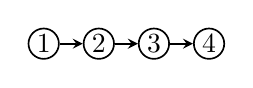
\begin{tikzpicture}[> = stealth, % arrow head style
                % shorten > = 1pt, % don't touch arrow head to node
                auto, node distance = 7mm, % distance between nodes
                semithick % line style
            ]

            \tikzstyle{every node}=[draw = black, circle, inner sep = 1pt,
            minimum size = 0.1mm]

            \node (1) {$1$}; \node (2) [right of=1] {$2$}; \node (3) [right
                of=2] {$3$}; \node (4) [right of=3] {$4$};

            \path[->] (1) edge (2); \path[->] (2) edge (3); \path[->] (3) edge
            (4);
        \end{tikzpicture}
    $$

    Then
    $$E = \begin{pmatrix} 1 & -1 & 0 & 0\\ 0 & 1 & -1 & 0\\ 0 & 0 & 1 & -1\\ 0 & 0 & 0 & 1\\\end{pmatrix}$$
    and calculating we find that  $$B = \begin{pmatrix} -1 & -1 & -1 & -1 \\ 1 &
            0  & 0  & 0       \\ 0 & 1 & 0 & 0\\ 0 & 0 & 1 & 0\\\end{pmatrix}$$
    We then calculate the eigenvalues for $B$, which are shown in the
    appendix; we find that $M(A_4) := M(B) = 1$.
\end{example}

\begin{example}
    Consider the quiver $A_4$ given by
    $$                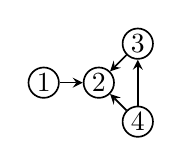
\begin{tikzpicture}[> = stealth, % arrow head style
                % shorten > = 1pt, % don't touch arrow head to node
                auto, node distance = 7mm, % distance between nodes
                semithick % line style
            ]

            \tikzstyle{every node}=[draw = black, circle, inner sep = 1pt,
            minimum size = 0.1mm]

            \node (1) {$1$}; \node (2) [right of=1] {$2$}; \node (3) [above
                right of=2] {$3$}; \node (4) [below right of=2] {$4$};

            \path[->] (1) edge (2); \path[->] (3) edge (2); \path[->] (4) edge
            (2); \path[->] (4) edge (3);
        \end{tikzpicture}
    $$

    Then
    $$E = \begin{pmatrix} 1 & -1 & 0 & 0\\ 0 & 1 & 0 & 0\\ 0 & -1 & 1 & 0\\ 0 & -1 & -1 & 1\\\end{pmatrix}$$
    and calculating we find that  $$B = \begin{pmatrix} -1 & -1 & 0 & 0 \\ 1 & 3
               & 2  & 1     \\ 0 & 1 & 0 & 1\\ 0 & -2 & -1 & -1\\\end{pmatrix}$$
    We then calculate the eigenvalues for $B$, which are plotted on
    the complex plane below:\\

    $$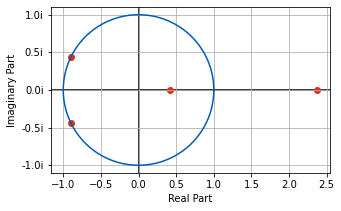
\includegraphics[scale=0.5]{pendulum4.png}$$

    We can see that two of the eigenvalues are not on the unit circle;
    calculating, we find that $M(B) \approx 2.3692054071$.
\end{example}

\section*{Goal and Approach}

This project will study the eigenvalues of $B$ in relation to their distance
from the unit circle. We will consider only connected quivers that do not
contain any oriented cycles.

\begin{question}
    If the eigenvalues of $B$ are not on the unit circle, how many are not on
    the unit circle, and how close are they to the unit circle?
\end{question}

This ties directly into \textit{Lehmer's Conjecture} or \textit{Lehmer's
    Question}:

\begin{question} Does there exist some $C > 1$ such that for every polynomial
    $P(x) \in \mathbb{Z}[x]$, $M(P) = 1$ or $M(P) > C$ \cite{m}?
\end{question}
Lehmer conjectured that $C \approx 1.1762808$, given by $M(P)$ for $P(x) =
    x^{10} + x^9 - x^7 - x^6 - x^5 - x^4 - x^3 + x + 1$ \cite{m}. Our approach
will use the properties of $E$ to derive properties of $B$ and $B$'s
eigenvalues. Currently, three questions are of particular interest:

\begin{question}
    Which polynomials $P$ can be written as the characteristic polynomial of a
    matrix $B$ such that $B = - E^T E^{-1}$ for some Euler Matrix $E$ of a
    quiver?
\end{question}

\begin{question}
    Given two quivers $Q$ and $Q'$, if $Q$ is a subgraph of $Q'$, is $M(Q) \leq
        (Q')$?
\end{question}

\begin{question}
    Does there exist a set of quivers $F = \{F_1, F_2, \dots F_m\}$ such that
    for all $i$, $M(F_i) > 1$ and any quiver $Q$ with $M(Q) > 1$ contains some
    $F_i$ as a subgraph?
\end{question}

The idea is hopefully to show that any polynomial that could have Mahler Measure
smaller than Lehmer's polynomial could be represented as the characteristic
polynomial of some $B$. Then, if all quivers with $M(Q) > 1$ have a subgraph
$F_i$ with $M(F_i) > 1$, and the set $F$ has some minimum $M(F_j)$, then that
would show that all polynomials have Mahler Measure greater than $\approx
    1.1762808$.

\section*{Background}

Lehmer first introduced his question in the 1933 paper \textit{Factorization of
    Certain Cyclotomic Functions} \cite{l}. The initial paper was motivated by
an approach for finding large primes \cite{ln}. A lemma of Kronecker implies
that if $M(P) = 1$, then $P$ is a product of powers of $x$ and cyclotomic
polynomials \cite{ln}.

Some partial results bounding Mahler measure have been established. Breusch
proved in 1951 that a monic, irreducible, and nonreciprocal polynomial $P$ then
$$M(P) \geq 1.324717\dots$$ which is the real root of $x^3 - x - 1$ \cite{ln}.
Later, in 1979, Dobrowolski showed that for a monic, irreducible, and
non-cyclotomic $P$,
$$M(P) > 1 + c \left(\frac{\log \log d}{\log d}\right)^3$$ for some constant $c$
\cite{ln}.

Several computational searches have been carried out in addition to the above
approaches. None have yielded a counterexample to Lehmer's question \cite{m}.
Mossinghoff carried out a search for all polynomials of degree at most 24 with
Mahler measure less than 1.3; while the specific algorithm used applied only to
even degrees, he was able to find 48 such polynomials of degree 22 and 46 of
degree 24 \cite{m}. He was additionally able to use several other algorithms to
extend the search calculations to more degrees, and was able to find a limit
point for measures near 1.309 \cite{m}.

For more information on the work around Lehmer's question, see the cited works
\textit{Mahler Measure of Polynomials} and \textit{Polynomials with Small Mahler
    Measure}.

\section*{Examples}

This section contains a table of quivers, their matrices $B$, and plots of the
eigenvalues of $B$ in the complex plane. First, we have the simply laced Dynkin
diagrams.

\setlength\LTleft{-0.75in} \setlength\LTright{-1in}
\tiny
\begin{longtable}[H]{|c|c|c|}
    \hline
    \rule{0pt}{3ex}\centered{Graph}         & \centered{$B = -E^{T} E^{-1}$}                 &
    \centered{Plot of Eigenvalues of
        $B$}
    \\
    \hline
    % Dynkin diagrams
    \centered{
        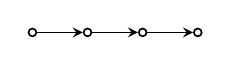
\begin{tikzpicture}[> = stealth, % arrow head style
                % shorten > = 1pt, % don't touch arrow head to node
                auto, node distance = 7mm, % distance between nodes
                semithick % line style
            ]

            \tikzstyle{every node}=[draw = black, circle, inner sep = 1pt,
            minimum size = 0.1mm]

            \node (1) {}; \node (2) [right of=1] {}; \node (3) [right of=2] {};
            \node (4) [right of=3] {};

            \path[->] (1) edge (2); \path[->] (2) edge (3); \path[->] (3) edge
            (4);
        \end{tikzpicture}
    }                                       & \centered{$\begin{pmatrix} -1 & -1
                   & -1 & -1 \\ 1 & 0 & 0 & 0\\ 0 & 1 & 0 & 0\\ 0 & 0 & 1 & 0
                \\\end{pmatrix}$}        &
    \centered{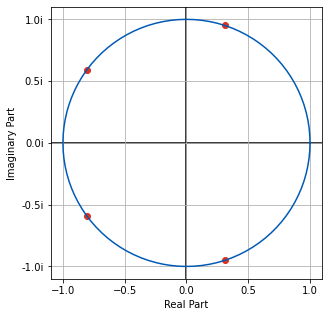
\includegraphics[scale=0.3]{a4.png}}                                                 \\
    \hline
    \centered{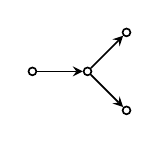
\begin{tikzpicture}[> = stealth, % arrow head style
                % shorten > = 1pt, % don't touch arrow head to node
                auto, node distance = 7mm, % distance between nodes
                semithick % line style
            ]

            \tikzstyle{every node}=[draw = black, circle, inner sep = 1pt,
            minimum size = 0.1mm]

            \node (1) {}; \node (2) [right of=1] {}; \node (3) [above right
                of=2] {}; \node (4) [below right of=2] {};

            \path[->] (1) edge (2); \path[->] (2) edge (4); \path[->] (2) edge
            (3); \end{tikzpicture}}   & \centered{$\begin{pmatrix} -1 & -1 & -1
                   & -1      \\ 1 & 0 & 0 & 0\\ 0 & 1 & 0 & 0\\ 0 & 0 & 1 & 0
                \\\end{pmatrix}$}        &
    \centered{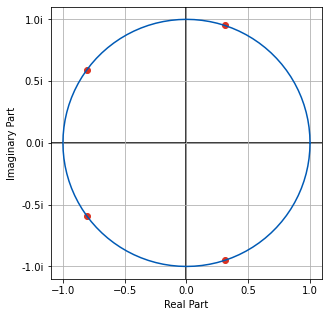
\includegraphics[scale=0.3]{d4.png}}                                             \\
    \hline
    \centered{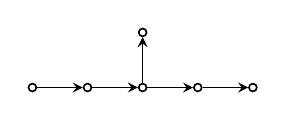
\begin{tikzpicture}[> = stealth, % arrow head style
                % shorten > = 1pt, % don't touch arrow head to node
                auto, node distance = 7mm, % distance between nodes
                semithick % line style
            ]

            \tikzstyle{every node}=[draw = black, circle, inner sep = 1pt,
            minimum size = 0.1mm]

            \node (1) {}; \node (2) [right of=1] {}; \node (3) [right of=2] {};
            \node (4) [above of=3] {}; \node (5) [right of=3] {}; \node (6)
            [right of=5] {};


            \path[->] (1) edge (2); \path[->] (2) edge (3); \path[->] (3) edge
            (4); \path[->] (3) edge (5); \path[->] (5) edge (6);
        \end{tikzpicture}}   & \centered{$\begin{pmatrix} -1 & -1 & -1 & -1
                   & -1 & -1 &              \\ 1 & 0 & 0 & 0 & 0 & 0 & \\ 0 & 1 & 0 & 0
                   & 0  & 0  &              \\
                0  & 0  & 1  & 0  & 1 & 1 & \\ 0 & 0 & 1 & 1 & 0 & 0 & \\ 0 & 0
                   & 0  & 0  & 1  & 0 &     \\
            \end{pmatrix}$}        &
    \centered{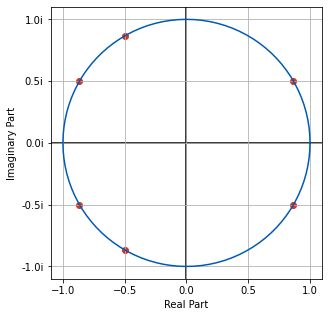
\includegraphics[scale=0.3]{e6.png}}                                             \\
    \hline
    \centered{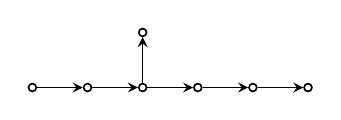
\begin{tikzpicture}[> = stealth, % arrow head style
                % shorten > = 1pt, % don't touch arrow head to node
                auto, node distance = 7mm, % distance between nodes
                semithick % line style
            ]

            \tikzstyle{every node}=[draw = black, circle, inner sep = 1pt,
            minimum size = 0.1mm]

            \node (1) {}; \node (2) [right of=1] {}; \node (3) [right of=2] {};
            \node (4) [above of=3] {}; \node (5) [right of=3] {}; \node (6)
            [right of=5] {}; \node (7) [right of=6] {};


            \path[->] (1) edge (2); \path[->] (2) edge (3); \path[->] (3) edge
            (4); \path[->] (3) edge (5); \path[->] (5) edge (6); \path[->] (6)
            edge (7); \end{tikzpicture}}   & \centered{$\begin{pmatrix} -1 & -1
                   & -1 & -1 & -1 & -1 & -1 & \\ 1 & 0 & 0 & 0 & 0 & 0 & 0 & \\ 0 & 1 &
                0  & 0  & 0  & 0  & 0  &      \\ 0 & 0 & 1 & 0 & 1 & 1 & 1 & \\ 0 &
                0  & 1  & 1  & 0  & 0  & 0  & \\ 0 & 0 & 0 & 0 & 1 & 0 & 0 & \\ 0 &
                0  & 0  & 0  & 0  & 1  & 0  & \\
            \end{pmatrix}$}        &
    \centered{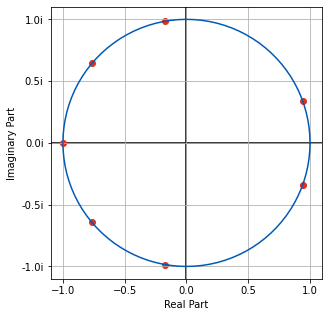
\includegraphics[scale=0.3]{e7.png}}                                             \\
    \hline
    \centered{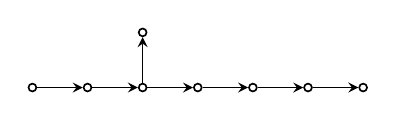
\begin{tikzpicture}[> = stealth, % arrow head style
                % shorten > = 1pt, % don't touch arrow head to node
                auto, node distance = 7mm, % distance between nodes
                semithick % line style
            ]

            \tikzstyle{every node}=[draw = black, circle, inner sep = 1pt,
            minimum size = 0.1mm]

            \node (1) {}; \node (2) [right of=1] {}; \node (3) [right of=2] {};
            \node (4) [above of=3] {}; \node (5) [right of=3] {}; \node (6)
            [right of=5] {}; \node (7) [right of=6] {}; \node (8) [right of=7]
            {};


            \path[->] (1) edge (2); \path[->] (2) edge (3); \path[->] (3) edge
            (4); \path[->] (3) edge (5); \path[->] (5) edge (6); \path[->] (6)
            edge (7); \path[->] (7) edge (8); \end{tikzpicture}}   &
    \centered{$\begin{pmatrix} -1 & -1 & -1 & -1 & -1 & -1 & -1 & -1 &
                \\ 1 & 0 & 0 & 0 & 0 & 0 & 0 & 0 & \\ 0 & 1 & 0 & 0 & 0 & 0 & 0 & 0
                   &                                    \\ 0 & 0 & 1 & 0 & 1 & 1 & 1 &
                1  &                                    \\ 0 & 0 & 1 & 1 & 0 & 0 & 0
                   & 0  &                               \\ 0 & 0 & 0 & 0 & 1 & 0 & 0 &
                0  &                                    \\ 0 & 0 & 0 & 0 & 0 & 1 & 0  & 0  &
                \\ 0 & 0 & 0 & 0 & 0 & 0 & 1  & 0  &                          \\
            \end{pmatrix}$} & \centered{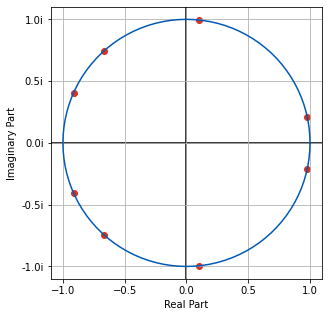
\includegraphics[scale=0.3]{e8.png}}   \\
    \hline
    \caption{\textit{ADE}-quivers and roots of $B$}
    \label{tab:ade}
\end{longtable}

\normalsize
Next we have the extended Dynkin diagrams.

\tiny
\begin{longtable}[H]{|c|c|c|}
    \hline
    \rule{0pt}{3ex}\centered{Graph}         & \centered{$B = -E^{T} E^{-1}$}                     &
    \centered{Plot of Eigenvalues of
        $B$}
    \\
    \hline
    % Extended Dynkin Diagrams
    \centered{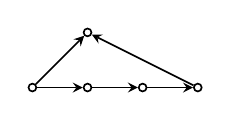
\begin{tikzpicture}[> = stealth, % arrow head style
                % shorten > = 1pt, % don't touch arrow head to node
                auto, node distance = 7mm, % distance between nodes
                semithick % line style
            ]

            \tikzstyle{every node}=[draw = black, circle, inner sep = 1pt,
            minimum size = 0.1mm]

            \node (1) {}; \node (2) [right of=1] {}; \node (3) [right of=2] {};
            \node (4) [right of=3] {}; \node (5) [above of=2] {};


            \path[->] (1) edge (2); \path[->] (2) edge (3); \path[->] (3) edge
            (4); \path[->] (4) edge (5); \path[->] (1) edge (5);
        \end{tikzpicture}}   &

    \centered{$\begin{pmatrix} -1 & -1 & -1 & -1 & -2 & \\ 1 & 0 & 0 & 0 & 1 &
                \\ 0 & 1 & 0 & 0 & 0 & \\ 0 & 0 & 1 & 0 & 0 & \\ 1 & 1 & 1 & 2 &
                2  &                     \\
            \end{pmatrix}$} & \centered{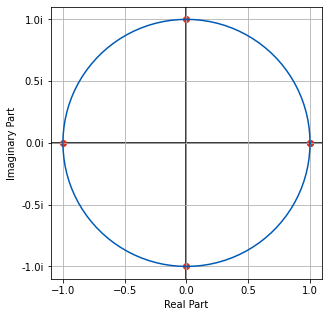
\includegraphics[scale=0.3]{a4_ext.png}}
    \\
    \hline
    \centered{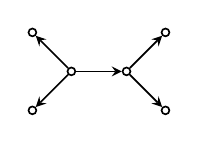
\begin{tikzpicture}[> = stealth, % arrow head style
                % shorten > = 1pt, % don't touch arrow head to node
                auto, node distance = 7mm, % distance between nodes
                semithick % line style
            ]

            \tikzstyle{every node}=[draw = black, circle, inner sep = 1pt,
            minimum size = 0.1mm]

            \node (1) {}; \node (2) [right of=1] {}; \node (3) [above right
                of=2] {}; \node (4) [below right of=2] {}; \node (5) [above left
                of=1] {}; \node (6) [below left of=1] {};


            \path[->] (1) edge (2); \path[->] (2) edge (3); \path[->] (2) edge
            (4); \path[->] (1) edge (5); \path[->] (1) edge (6);
        \end{tikzpicture}}   &

    \centered{$\begin{pmatrix} -1 & -1 & -1 & -1 & -1 & -1 & \\ 1 & 0 & 0 & 0 &
                0  & 0  &                     \\ 0 & 1 & 0 & 0 & 0 & 1 & \\ 0 &
                0  & 1  & 0  & 1  & 0  &      \\ 0 & 0 & 1 & 1  & 0  & 0  & \\ 0
                   & 1  & 1  & 1  & 1  & 0  & \\
            \end{pmatrix}$} & \centered{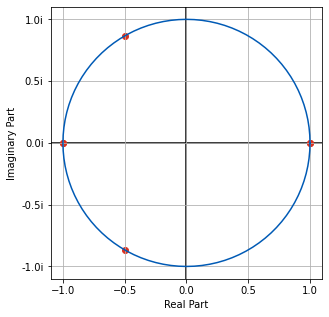
\includegraphics[scale=0.3]{d4_ext.png}}
    \\
    \hline
    \centered{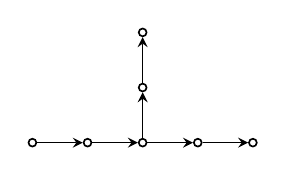
\begin{tikzpicture}[> = stealth, % arrow head style
                % shorten > = 1pt, % don't touch arrow head to node
                auto, node distance = 7mm, % distance between nodes
                semithick % line style
            ]

            \tikzstyle{every node}=[draw = black, circle, inner sep = 1pt,
            minimum size = 0.1mm]

            \node (1) {}; \node (2) [right of=1] {}; \node (3) [right of=2] {};
            \node (4) [above of=3] {}; \node (5) [above of=4] {}; \node (6)
            [right of=3] {}; \node (7) [right of=6] {};


            \path[->] (1) edge (2); \path[->] (2) edge (3); \path[->] (3) edge
            (4); \path[->] (4) edge (5); \path[->] (3) edge (6); \path[->] (6)
            edge (7); \end{tikzpicture}}   &

    \centered{$\begin{pmatrix} -1 & -1 & -1 & -1 & -1 & -1 & -1 & \\ 1 & 0 & 0 &
                0  & 0  & 0  & 0  &                \\ 0 & 1 & 0 & 0 & 0 & 0 & 0
                   &                               \\ 0 & 0 & 1 & 0 & 1 & 1 & 0 &
                \\ 0 & 0  & 1  & 1  & 0  & 0  & 1  &      \\ 0 & 0 & 0  & 0  & 1
                   & 0  & 0  &                     \\ 0 & 0 & 0 & 1 & 0  & 0  & 0  & \\
            \end{pmatrix}$} & \centered{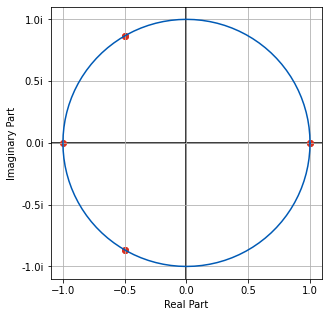
\includegraphics[scale=0.3]{e6_ext.png}}
    \\
    \hline
    \centered{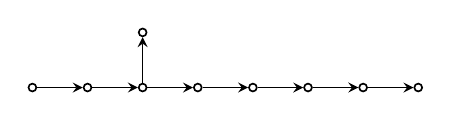
\begin{tikzpicture}[> = stealth, % arrow head style
                % shorten > = 1pt, % don't touch arrow head to node
                auto, node distance = 7mm, % distance between nodes
                semithick % line style
            ]

            \tikzstyle{every node}=[draw = black, circle, inner sep = 1pt,
            minimum size = 0.1mm]

            \node (1) {}; \node (2) [right of=1] {}; \node (3) [right of=2] {};
            \node (4) [above of=3] {}; \node (5) [right of=3] {}; \node (6)
            [right of=5] {}; \node (7) [right of=6] {}; \node (8) [right of=7]
            {}; \node (9) [right of=8] {};


            \path[->] (1) edge (2); \path[->] (2) edge (3); \path[->] (3) edge
            (4); \path[->] (3) edge (5); \path[->] (5) edge (6); \path[->] (6)
            edge (7); \path[->] (7) edge (8); \path[->] (8) edge (9);
        \end{tikzpicture}}   & \centered{$\begin{pmatrix} -1 & -1 & -1 & -1 &
                -1 & -1 & -1 & -1 & -1 &                 \\
                1  & 0  & 0  & 0  & 0  & 0 & 0 & 0 & 0 & \\ 0 & 1 & 0 & 0 &
                0  & 0  & 0  & 0  & 0  &                 \\ 0 & 0 & 1 & 0 & 1 & 1 & 1 & 1 & 1 & \\ 0
                   & 0  & 1  & 1  & 0  & 0 & 0 & 0 & 0 &
                \\ 0 & 0 & 0 & 0 & 1 & 0 & 0 & 0 & 0 & \\ 0 & 0 & 0 & 0 & 0 & 1
                   & 0  & 0  & 0  &                      \\ 0 & 0
                   & 0  & 0  & 0  & 0  & 1 & 0 & 0 &     \\ 0 & 0 & 0 & 0 & 0 & 0 & 0 & 1 &
                0  &                                     \\
            \end{pmatrix}$}            &
    \centered{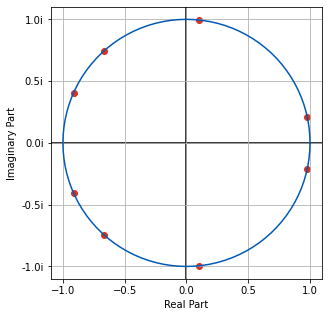
\includegraphics[scale=0.3]{e8.png}}
    \\
    \hline
    \caption{Extended \textit{ADE}-quivers and roots of $B$}
    \label{tab:ade}
\end{longtable}

\normalsize
Finally, we show an example of a sequence of quivers such that the quiver in
each row is a subquiver of the following rows.

\tiny
\begin{longtable}[H]{|c|c|c|}
    \hline
    \rule{0pt}{3ex}\centered{Graph}         & \centered{$B = -E^{T} E^{-1}$}          &
    \centered{Plot of Eigenvalues of
        $B$}
    \\
    \hline
    % "Pendulum" example with sequence of subquivers
    \centered{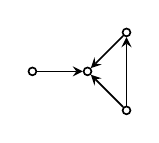
\begin{tikzpicture}[> = stealth, % arrow head style
                % shorten > = 1pt, % don't touch arrow head to node
                auto, node distance = 7mm, % distance between nodes
                semithick % line style
            ]

            \tikzstyle{every node}=[draw = black, circle, inner sep = 1pt,
            minimum size = 0.1mm]

            \node (1) {}; \node (2) [right of=1] {}; \node (3) [above right
                of=2] {}; \node (4) [below right of=2] {};

            \path[->] (1) edge (2); \path[->] (4) edge (2); \path[->] (3) edge
            (2); \path[->] (4) edge (3); \end{tikzpicture}}   &
    \centered{$\begin{pmatrix} -1 & -1 & 0 & 0 & \\ 1 & 3 & 2 & 1 & \\ 0
                   & 1  & 0 & 1 & \\ 0 & -2 & -1 & -1 & \\
            \end{pmatrix}$} &
    \centered{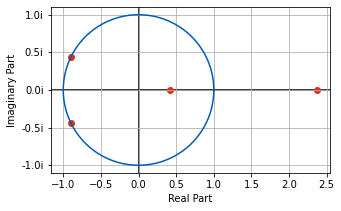
\includegraphics[scale=0.3]{pendulum4.png}}                               \\
    \hline

    \centered{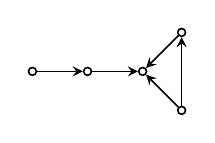
\begin{tikzpicture}[> = stealth, % arrow head style
                % shorten > = 1pt, % don't touch arrow head to node
                auto, node distance = 7mm, % distance between nodes
                semithick % line style
            ]

            \tikzstyle{every node}=[draw = black, circle, inner sep = 1pt,
            minimum size = 0.1mm]

            \node (1) {}; \node (2) [right of=1] {}; \node (3) [above right
                of=2] {}; \node (4) [below right of=2] {}; \node (5) [left of=1]
            {};

            \path[->] (1) edge (2); \path[->] (4) edge (2); \path[->] (3) edge
            (2); \path[->] (4) edge (3); \path[->] (5) edge (1);
        \end{tikzpicture}}   & \centered{$\begin{pmatrix} 0  & 0  & 0 & 0 & 1
                   &                \\ 1 & 3 & 2 & 1 & 0 & \\ 0 & 1 & 0 & 1 & 0 & \\ 0 & -2 &
                -1 & -1 & 0 &       \\ -1 & -1 & 0 & 0 & -1 & \\
            \end{pmatrix}$} &
    \centered{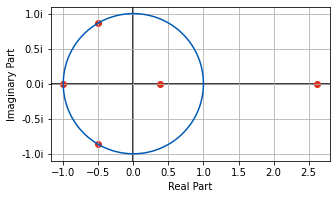
\includegraphics[scale=0.3]{pendulum5.png}}
    \\
    \hline

    \centered{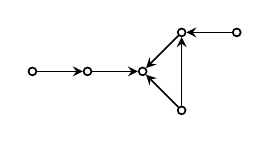
\begin{tikzpicture}[> = stealth, % arrow head style
                % shorten > = 1pt, % don't touch arrow head to node
                auto, node distance = 7mm, % distance between nodes
                semithick % line style
            ]

            \tikzstyle{every node}=[draw = black, circle, inner sep = 1pt,
            minimum size = 0.1mm]

            \node (1) {}; \node (2) [right of=1] {}; \node (3) [above right
                of=2] {}; \node (4) [below right of=2] {}; \node (5) [left of=1]
            {}; \node (6) [right of=3] {};

            \path[->] (1) edge (2); \path[->] (4) edge (2); \path[->] (3) edge
            (2); \path[->] (4) edge (3); \path[->] (5) edge (1); \path[->] (6)
            edge (3);\end{tikzpicture}}   & \centered{$\begin{pmatrix} -1 & -1 &
                0  & 0  & 0  & 0 & \\ 1 & 3 & 2 & 1 & 0 & 0 & \\ 0 & 3 & 2 & 1 & 1 & 1
                   &               \\ 0 & -2 & -1 & -1 & 0 & 0  & \\ 0 & -1 & -1
                   & 0  & -1 & 0 & \\ 0 & -1 & -1 & 0 & 0 & -1 & \\
            \end{pmatrix}$} &
    \centered{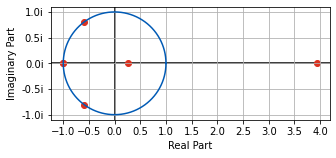
\includegraphics[scale=0.3]{pendulum6.png}}
    \\
    \hline


    \centered{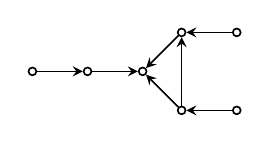
\begin{tikzpicture}[> = stealth, % arrow head style
                % shorten > = 1pt, % don't touch arrow head to node
                auto, node distance = 7mm, % distance between nodes
                semithick % line style
            ]

            \tikzstyle{every node}=[draw = black, circle, inner sep = 1pt,
            minimum size = 0.1mm]

            \node (1) {}; \node (2) [right of=1] {}; \node (3) [above right
                of=2] {}; \node (4) [below right of=2] {}; \node (5) [left of=1]
            {}; \node (6) [right of=3] {}; \node (7) [right of=4] {};

            \path[->] (1) edge (2); \path[->] (4) edge (2); \path[->] (3) edge
            (2); \path[->] (4) edge (3); \path[->] (5) edge (1); \path[->] (6)
            edge (3); \path[->] (7) edge (4); \end{tikzpicture}}   &
    \centered{$\begin{pmatrix} -1 & -1 & 0 & 0 & 0 & 0 & 0 &
                \\ 1 & 3 & 2 & 1 & 0 & 0 & 0 & \\ 0 & 3 & 2 & 1 & 1 & 1 & 0 & \\ 0 &
                0  & 0  & 0 & 0 & 0 & 1 &     \\ 0 & -1 & -1 & 0 & -1 & 0 & 0 &
                \\ 0 & -1 & -1 & 0 & 0 & -1 & 0  & \\ 0 & -2 & -1 & -1 & 0 & 0 & -1 & \\
            \end{pmatrix}$} &
    \centered{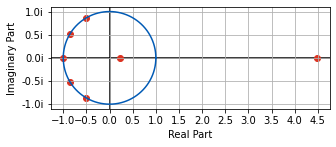
\includegraphics[scale=0.3]{pendulum7.png}}
    \\
    \hline

    \caption{"Pendulum" quiver sequence and roots of $B$}
    \label{tab:ade}
\end{longtable}
\normalsize

\section*{Works In Progress}

This section contains some current remarks and propositions that have not been categorized into the
rest of the paper. 

\begin{proposition}
    Any polyonomial with common factor $a_d > 1$ cannot have $M(P)$ less than the Salem number.
    \begin{proof}
        Consider some $P(x) = a_d \prod_{i=1}^{n} (x - \alpha_i)$ where $a_d > 1$. Since $P$ has coefficients
        in the integers, $a_d$ is an integer. Then $a_d \geq 2$, and by the definition of Mahler measure
        $$M(P) = |a_d| \prod_{i=1}^{n} \max\{1, |\alpha_i|\}$$ so $M(P) \geq 2$.
    \end{proof}
\end{proposition}

As a result of this proposition, we can see that we need only to concern ourselves with polynomials that
have $a_d = 1$. This is good news, as the characteristic polynomials of $B$ do in fact
have $a_d = 1$ (I think I showed this earlier).

We can also start to bound the entries of $E^{-1}$ based on facts about triangular matrices:

\begin{proposition}
    For a matrix $E$ of a quiver with no self-loops, the diagonal entries of
    $E^T$ are 1 and the diagonal entries of $E^{-1}$ are $\pm 1$.
    \begin{proof}
        Since we know that $\det E = 1$, $E$ is triangular, and for a quiver with
        no self-loops, the diagonal entries of $E$ are 1. So the diagonal entries
        of $E^T$ are also 1. Since we know that $E$ is triangular,
        we know that $E^{-1}$ is also triangular, and since we know that
        $\det E^{-1} = 1$, the diagonal entries of $E^{-1}$ must have product 1.
        Furthermore, since $E$ is defined as having integer entries and has 
        determinant 1, $E^{-1}$ has integer entries, which means that the diagonal
        values of $E^{-1}$ are $\pm 1$. 
    \end{proof}
\end{proposition}

\begin{thebibliography}{99}

    \bibitem{dw} Derksen, H., Weyman, J., {\em An Introduction to Quiver
            Representations\/}, American Mathematical Society, Providence,
    Graduate Studies in Mathematics. {\bf 52} (2017), 1-33.

    \bibitem{m} Mossinghoff, M. J. {\em Polynomials with Small Mahler
            Measure\/}, Mathematics of Computation. {\bf 67} (1998), 1697-1705.

    \bibitem{l} Lehmer, D. H. {\em Factorization of Certain Cyclotomic
            Functions\/}, Annals of Mathematics. {\bf 34} (1933), 461-479.

    \bibitem{ln} Lalin, Matilde N. {\em Mahler Measure of Polynomials\/}
    Postdoctoral Seminar, Mathematical Sciences Research Institute. (2006), 1-2.

\end{thebibliography}
\pagebreak

\appendix

\section{Source Code}

This section contains the code used to generate matrices and eigenvalue plots.

\lstinputlisting[language=Python]{matrix_calculations.py}

\end{document}